The general second order equation can be expressed as follows,
\begin{align}
\vec{x^T}\vec{V}\vec{x}+2\vec{u^T}\vec{x}+f=0\label{eq:solutions/3/4/6/eq:eq1}
\end{align}
Comparing \eqref{eq:solutions/3/4/6/eq:q1} with \eqref{eq:solutions/3/4/6/eq:eq1},
\begin{align}
\vec{V} &= \myvec{1 & 2\\2 & -2}\\
\vec{u} &= \myvec{5\\ -2}\\
f &= 0
\end{align}
Let the point to which the origin is moved be $\vec{c}$\\
The above equation \eqref{eq:solutions/3/4/6/eq:eq1} can be modified as
\begin{align}
(\vec{x}+\vec{c})^T\vec{V}(\vec{x}+\vec{c})+2\vec{u}^T(\vec{x}+\vec{c})&=0\label{eq:solutions/3/4/6/eq:eq2}
\end{align}
From equation \eqref{eq:solutions/3/4/6/eq:eq2} consider,
\begin{align}
    &\implies(\vec{x}+\vec{c})^T\vec{V}(\vec{x}+\vec{c})\\
    &\implies\vec{x}^T\vec{V}\vec{x}+\vec{c}^T\vec{V}\vec{x}+\vec{x}^T\vec{V}\vec{c}+\vec{c}^T\vec{V}\vec{c}\label{eq:solutions/3/4/6/eq:eq3}\\
    &\implies\vec{x}^T\vec{V}\vec{x}+2\vec{c}^T\vec{V}\vec{x}+\vec{c}^T\vec{V}\vec{c}\label{eq:solutions/3/4/6/eq:eq4}
\end{align}
Substituting \eqref{eq:solutions/3/4/6/eq:eq4} in equation \eqref{eq:solutions/3/4/6/eq:eq2}
\begin{align}
    &\implies\vec{x}^T\vec{V}\vec{x}+2\vec{c}^T\vec{V}\vec{x}+\vec{c}^T\vec{V}\vec{c}+2\vec{u}^T(\vec{x}+\vec{c})=0 \label{eq:solutions/3/4/6/eq:eq5}
\end{align}
Comparing equations \eqref{eq:solutions/3/4/6/eq:eq5} and \eqref{eq:solutions/3/4/6/eq:q2}, we can write as,
\begin{align}
    &\implies 2\vec{c}^T\vec{V}\vec{x}+2\vec{u}^T\vec{x}=0\\
    &\implies \vec{c}^T\vec{V}= -\vec{u}^T\\
    &\implies \vec{c}= -\vec{V}^{-1}\vec{u}= -\myvec{\frac{1}{3}&\frac{1}{3}\\ \frac{1}{3}&-\frac{1}{6}}\myvec{5\\-2} \label{eq:solutions/3/4/6/eq:eq6}\\
    &\implies \boxed{\vec{c}= \myvec{-1\\-2}} \label{eq:solutions/3/4/6/eq:eq7}
\end{align}
From \eqref{eq:solutions/3/4/6/eq:eq7}, when the origin is moved to point $\vec{c}$, the equation \eqref{eq:solutions/3/4/6/eq:q1} becomes \eqref{eq:solutions/3/4/6/eq:q2}.\\
\\
From equations \eqref{eq:solutions/3/4/6/eq:q1} and \eqref{eq:solutions/3/4/6/eq:eq7}, $\vec{V}$ doesn't change
\begin{align}
    \det(\vec{V})&=-6
\end{align}
Since $\det(\vec{V})<0$ the given equation represents the hyperbola\\
\\
From equation \eqref{eq:solutions/3/4/6/eq:q2}, the equation is of the form,
\begin{align}
    \vec{x}^T\vec{V}\vec{x}+f=0
\end{align}
The matrix $\vec{V}$ can be decomposed as,
\begin{align}
    \vec{V} = \vec{P}\vec{D}\vec{P}^T \quad \vec{D}=\myvec{\lambda_1&0\\0&\lambda_2}
\end{align}
where $\lambda_1$ and $\lambda_2$ are Eigen values of $\vec{V}$, and $\vec{P}$ contains the Eigen vectors corresponding to the Eigen values $\lambda_1$ and $\lambda_2$. The affine transformation is given by,
\begin{align}
    \vec{x} = \vec{P}\vec{y}+\vec{c}
\end{align}
where, $\vec{P}$ indicates the rotation of axes and $\vec{c}$ indicates the shift of origin.\\
Eigen values of $\vec{V}$ are,
\begin{align}
   \mydet{\lambda\vec{I}-\vec{v}}=0\\
    \implies \mydet{\lambda-1&-2\\-2&\lambda+2}=0\\
    \implies \lambda^2+\lambda-6=0\\
    \implies \lambda_1=-3,\lambda_2=2\\
    \vec{D}=\myvec{-3&0\\0&2}
\end{align}
Eigen vector for $\lambda_1$=-3,
\begin{align}
    \lambda_1\vec{I}-\vec{v}=\myvec{-4&-2\\-2&-1}\xleftrightarrow[]{R_2\leftarrow R_2-\frac{R_1}{2}}\myvec{-2&-1\\0&0}\\
    \implies \vec{P_1}=\myvec{1\\-2}=\myvec{\frac{1}{\sqrt{5}}\\\frac{-2}{\sqrt{5}}}
\end{align}
Eigen vector for $\lambda_2$=2,
\begin{align}
    \lambda_1\vec{I}-\vec{v}=\myvec{1&-2\\-2&4}\xleftrightarrow[]{R_2\leftarrow R_2+2R_1}\myvec{1&-2\\0&0}\\
    \implies \vec{P_2}=\myvec{2\\1}=\myvec{\frac{2}{\sqrt{5}}\\\frac{1}{\sqrt{5}}}
\end{align}
\begin{align}
    \vec{P} = \myvec{\frac{1}{\sqrt{5}}&\frac{2}{\sqrt{5}}\\\frac{-2}{\sqrt{5}}&\frac{1}{\sqrt{5}}} \label{eq:solutions/3/4/6/eq:eq15}
\end{align}
Therefore $\vec{V}$ can be written as,
\begin{align}
    \vec{V}=\myvec{\frac{1}{\sqrt{5}}&\frac{2}{\sqrt{5}}\\\frac{-2}{\sqrt{5}}&\frac{1}{\sqrt{5}}}\myvec{-3&0\\0&2}\myvec{\frac{1}{\sqrt{5}}&\frac{-2}{\sqrt{5}}\\\frac{2}{\sqrt{5}}&\frac{1}{\sqrt{5}}}
\end{align}
Equation \eqref{eq:solutions/3/4/6/eq:q2} can be written as,
\begin{align}
    \vec{x}^T\left[\myvec{\frac{1}{\sqrt{5}}&\frac{2}{\sqrt{5}}\\\frac{-2}{\sqrt{5}}&\frac{1}{\sqrt{5}}}\myvec{-3&0\\0&2}\myvec{\frac{1}{\sqrt{5}}&\frac{-2}{\sqrt{5}}\\\frac{2}{\sqrt{5}}&\frac{1}{\sqrt{5}}}\right]\vec{x}=1\\
  \left[\myvec{\frac{1}{\sqrt{5}}&\frac{-2}{\sqrt{5}}\\\frac{2}{\sqrt{5}}&\frac{1}{\sqrt{5}}}\vec{x}\right]^T\myvec{-3&0\\0&2}\left[\myvec{\frac{1}{\sqrt{5}}&\frac{-2}{\sqrt{5}}\\\frac{2}{\sqrt{5}}&\frac{1}{\sqrt{5}}}\vec{x}\right]= 1\label{eq:solutions/3/4/6/eq:eq11}
\end{align}
Consider the rotation transformation 
\begin{align}
  \vec{x}=\vec{P}\vec{y}\\
  \implies \vec{x}=\myvec{\frac{1}{\sqrt{5}}&\frac{2}{\sqrt{5}}\\\frac{-2}{\sqrt{5}}&\frac{1}{\sqrt{5}}}\vec{y}\\
  \vec{P}^{-1}\vec{x}=\vec{P}^{-1}\vec{P}\vec{y}\\
  \implies \vec{y}= \vec{P}^{-1}\vec{x}\\
  \text{But, }\vec{P}^{-1}=\vec{P}^T\\
  \implies \vec{y}=\myvec{\frac{1}{\sqrt{5}}&\frac{-2}{\sqrt{5}}\\\frac{2}{\sqrt{5}}&\frac{1}{\sqrt{5}}}\vec{x} \label{eq:solutions/3/4/6/eq:eq12}
\end{align}
Using \eqref{eq:solutions/3/4/6/eq:eq12} in \eqref{eq:solutions/3/4/6/eq:eq11}, the equation can be rewritten as
\begin{align}
     \vec{y}^T\myvec{-3&0\\0&2}\vec{y}=1 \label{eq:solutions/3/4/6/eq:eq13}
\end{align}
Equation \eqref{eq:solutions/3/4/6/eq:eq13} is same as \eqref{eq:solutions/3/4/6/eq:q3} with $p$=-3 and $q$=2.\\
From equation \eqref{eq:solutions/3/4/6/eq:eq15}, the orthogonal matrix represents the rotation matrix in form of,
\begin{align}
    \vec{P}=\myvec{\cos\theta & \sin\theta\\ -\sin\theta& \cos\theta} \label{eq:solutions/3/4/6/eq:eq16}
\end{align}
Comparing \eqref{eq:solutions/3/4/6/eq:eq15} and \eqref{eq:solutions/3/4/6/eq:eq16},
\begin{align}
    \cos\theta = \frac{1}{\sqrt{5}}\\
    \implies \boxed{\theta = 63.43^{\circ}}
\end{align}
From equation \eqref{eq:solutions/3/4/6/eq:eq16},if the axes is turned by $\theta$ then the equation obtained would be \eqref{eq:solutions/3/4/6/eq:q3}.
\begin{figure}[h!]
	\centering
	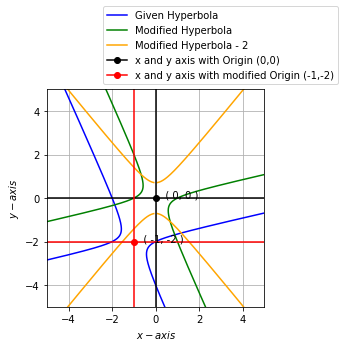
\includegraphics[width=\columnwidth]{./solutions/3/4/6/hyperbola.png}
	\caption{Hyperbola plot when origin is shifted and rotated}
	\label{eq:solutions/3/4/6/myfig}
\end{figure}
